% !TEX root = ../main.tex
%
\chapter{Standardized Data Collection}
\label{sec:data-collection}


\section{Background}

In urbanized environments, the high percentage of surface area covered in impermeable asphalt or buildings causes increased runoff and reduced evaporation and infiltration (Figure \ref{fig:urban-water-budget}).
Urban environments have long faced challenges when it comes to handling this increased runoff in a ecologically friendly manner that avoids disastrous flooding while also minimizing the impact to stream and river health from pollutants and erosive flow rates.
As cities' impervious footprints grow, sewer networks have became overwhelmed by the volumes seen during storm events, and outfall locations were added to avoid sewage backup into homes and streets.
In Philadelphia, combined sewer systems (CSS)  were the preferred method of handling large volumes of rainfall and sewage for nearly the city's entire history (\cite{Akhavan2015}), but have a major negative impact on the environment via combined sewer overflows (CSO).
The EPA's oversight of CSO events, outlined in the Clean Water Act of 1972 and regulated by the National Pollutant Discharge Elimination System (NPDES) permit program (\cite{USEPA2009}), require that cities address urban runoff and impose significant fines for overflow events.
Only recently have green initiatives such as Philadelphia's "Green City Clean Water" expanded, allowing the city to expedite the creation of environmentally friendly means of removing stormwater (\cite{PhiladelphiaWaterDepartment2018a, Callahan2019}).
These systems allow urban stormwater, which primarily falls on impervious surfaces and leads to increased runoff as compared to natural environments, to be captured and managed largely in place (\cite{Heffernan2016}) by a combination of green infrastructure methods including rain gardens, tree trenches, green roofs, and pervious concrete.
The type of system chosen for a particular site depends on existing site infrastructure (e.g., buried utilities, surrounding structures, etc.), grading, available space, and loading ratio (directly connected impervious area (DCIA) vs system footprint).

\begin{figure}[ht]
	\centering
	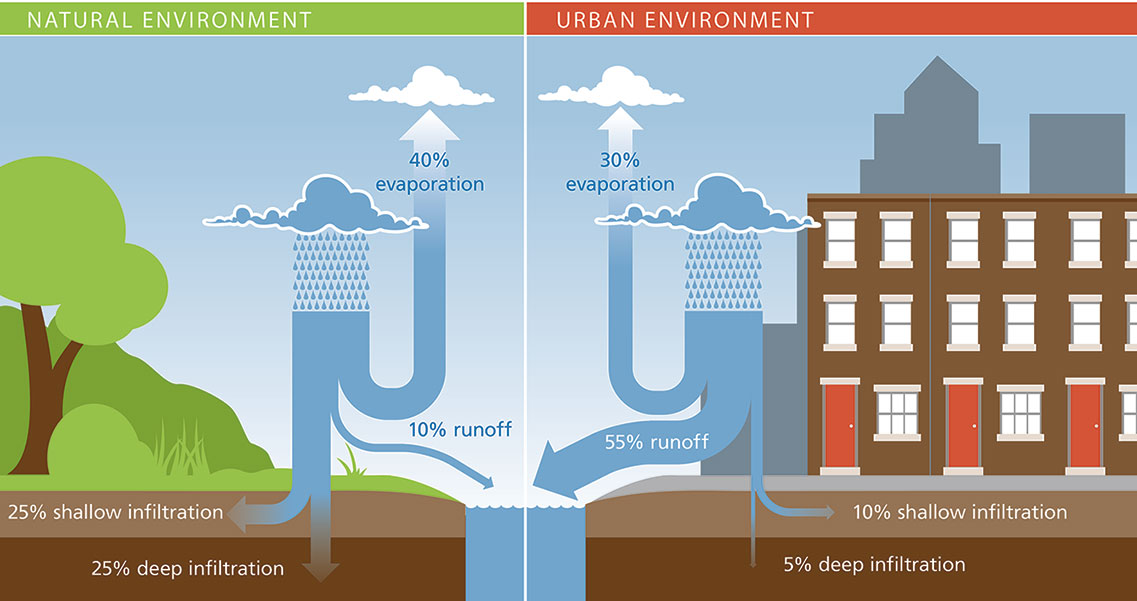
\includegraphics[width=0.8\textwidth]{gfx/chapter-instrumentation/naturalvsurbanrunoff.jpg}
	\caption[Natural vs Urban water budget.]{Natural vs Urban water budget (\cite{PhiladelphiaWaterDepartment2021}).}
	\label{fig:urban-water-budget}
\end{figure}

Measuring any natural or anthropogenic system is not without its challenges: atmospheric and physical parameters are subject to rapid change from weather patterns and equipment must be able to withstand harsh outdoor conditions for extended periods of time.
After all, nature obeys the laws of entropy, and energy tends to dissipate towards its lowest potential, and in doing so becomes a major force with which to be reckoned.
The water cycle that forms our climate is driven by solar heat inputs to this energy system.
Rainfall is generated from the accumulation of evaporated water in the atmosphere, which then condenses and falls to the ground.
Due to the randomness of entropy, no two storms will ever be the same in magnitude, duration, or intensity profile, so constructed solutions must be flexible enough to handle storms ranging from slow, drawn out events to short, intense events (\cite{Dourte2015, Maier2020}).

Collecting valid data is the first step to any rigorous experiment.
The methods used to collect this data must be reliable and easily repeatable for other parties who wish to replicate results.
That is to say identical inputs to a measurement system, given the same external conditions, should yield the same results.
This is a fundamental premise of the scientific method.
The most important aspects of monitoring a green stormwater infrastructure (GSI) system are a reliable data logger with minimal downtime, connected to a central data server (or "cloud") that collects data at a regular interval and redundantly stores that data for further analysis.
The data logger must be able to poll all connected sensors at timely intervals such that data measurements are associated with an accurate timestamp.
Measurements must be accurate, while their precision can be based on the unit of measure.
The ability to continuously monitor GSI conditions enables an understanding of design specifications versus real world performance.
While models are useful tools for understanding and managing expectations for GSI, they can only go so far at capturing real world knowledge and the many interactions of GSI conditions that create nearly endless combinations of unique conditions.

This chapter outlines a framework of best practices pertaining to the continuous remote sensing of GSI conditions developed for stormwater management practice (SMP) A in the GR2 section of the Pennsylvania Department of Transportation's (PennDOT) I-95 Girard Avenue Interchange Stormwater Project.
This framework has been developed to be reliable, consistent, easy to implement, and expandable to other GSI systems across Philadelphia with minimal additional configuration.
A primary goal of this research effort is to not only inform better data collection, but also to enable data to be collected at scale across many sites in a project or across many different projects.
A consistent, uniform framework for monitoring sites would allow for more widespread analysis of GSI's performance, maintenance needs, and impact on the natural environment (\cite{Burcin2014}).
This aligns well with the I-95 Girard Avenue Interchange Stormwater Project's long term horizon for construction, monitoring, and analysis of individual GSI systems and wider wholistic project or regional scale analysis.
A uniform approach across many individual sites ensures that statistical contrasts at the regional scale are accurate and unbiased.
To that end, measurements must be precise and data recording and transmission must be unhindered by the inherent randomness or other inconsistency of environmental systems.
Myriad challenges exist in monitoring GSI systems, but the focus of this discussion is accurate measurements of ponded and flowing water, which exhibits a wide variety of properties ranging from depth and velocity to random formations of currents and internal feedback in the form of turbulence (\cite{mays2010water}).
This monitoring framework has been established based on work performed at SMP A, a well developed and successfully performing GSI installation, for use across other PennDOT sites or for wider adoption across a regional scale in Philadelphia to enable long-term, meaningful comparisons of GSI performance across many systems.
The framework is intended as a basis for answering questions about ongoing maintenance requirements, identifying under-performing sites, and quantifying with high accuracy the environmental benefits of successful systems.

\section{Site Configuration}
Situated along the south side of Interstate 95 northbound, SMP A handles inflow from the elevated roadway surface's rainfall runoff that flows through a network of pipes beneath the highway.
Most of the DCIA lies in the northbound highway section, per LiDAR surveys conducted in 2017.
SMP A is a linear bioswale type rain garden split into three sections by two check dams placed at roughly the third points of the garden (Figure \ref{fig:site-layout}).

\begin{figure}[ht!]
	\centering
	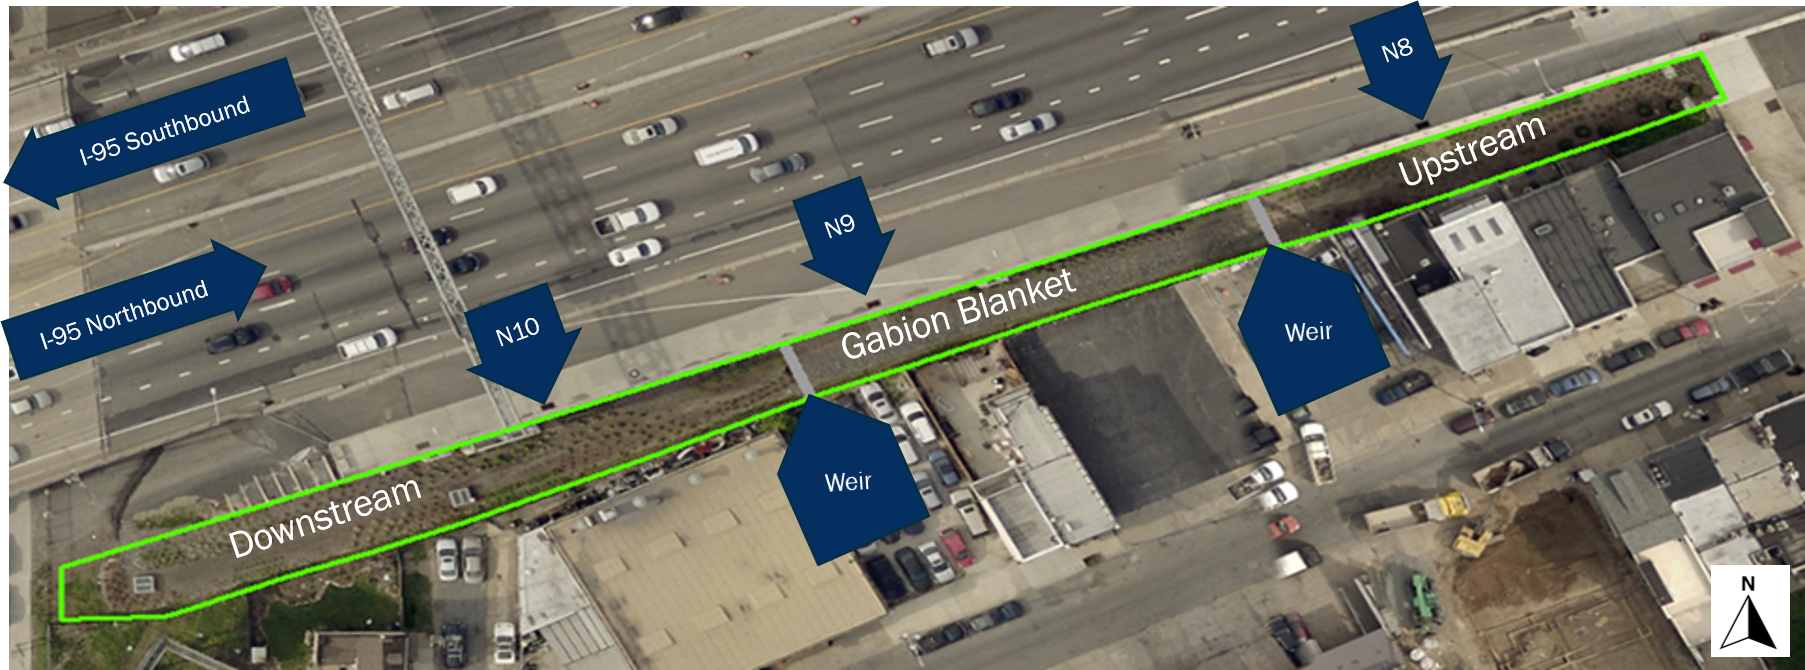
\includegraphics[width=0.8\textwidth]{gfx/chapter-instrumentation/site-layout.png}
	\caption{SMP A site layout.}
	\label{fig:site-layout}
\end{figure}

The upstream portion contains one inlet (N8) that is a 76.2cm diameter reinforced concrete pipe (RCP).
This upstream section is planted with local, salt tolerant grasses and small coniferous trees.
The surface is mulched during annual maintenance cycles, and the cross-sectional geometry is gently sloping (Figure \ref{fig:us-profile}).
The upstream section terminates with a 45\degree\ steel weir plate situated in the center of a plywood check dam that reduces flow rates, encourages infiltration by retaining some water, and measures inter-garden flow once overtopped using the standard weir equation (Figure \ref{fig:check-dam}).

\begin{figure}[ht!]
	\centering
	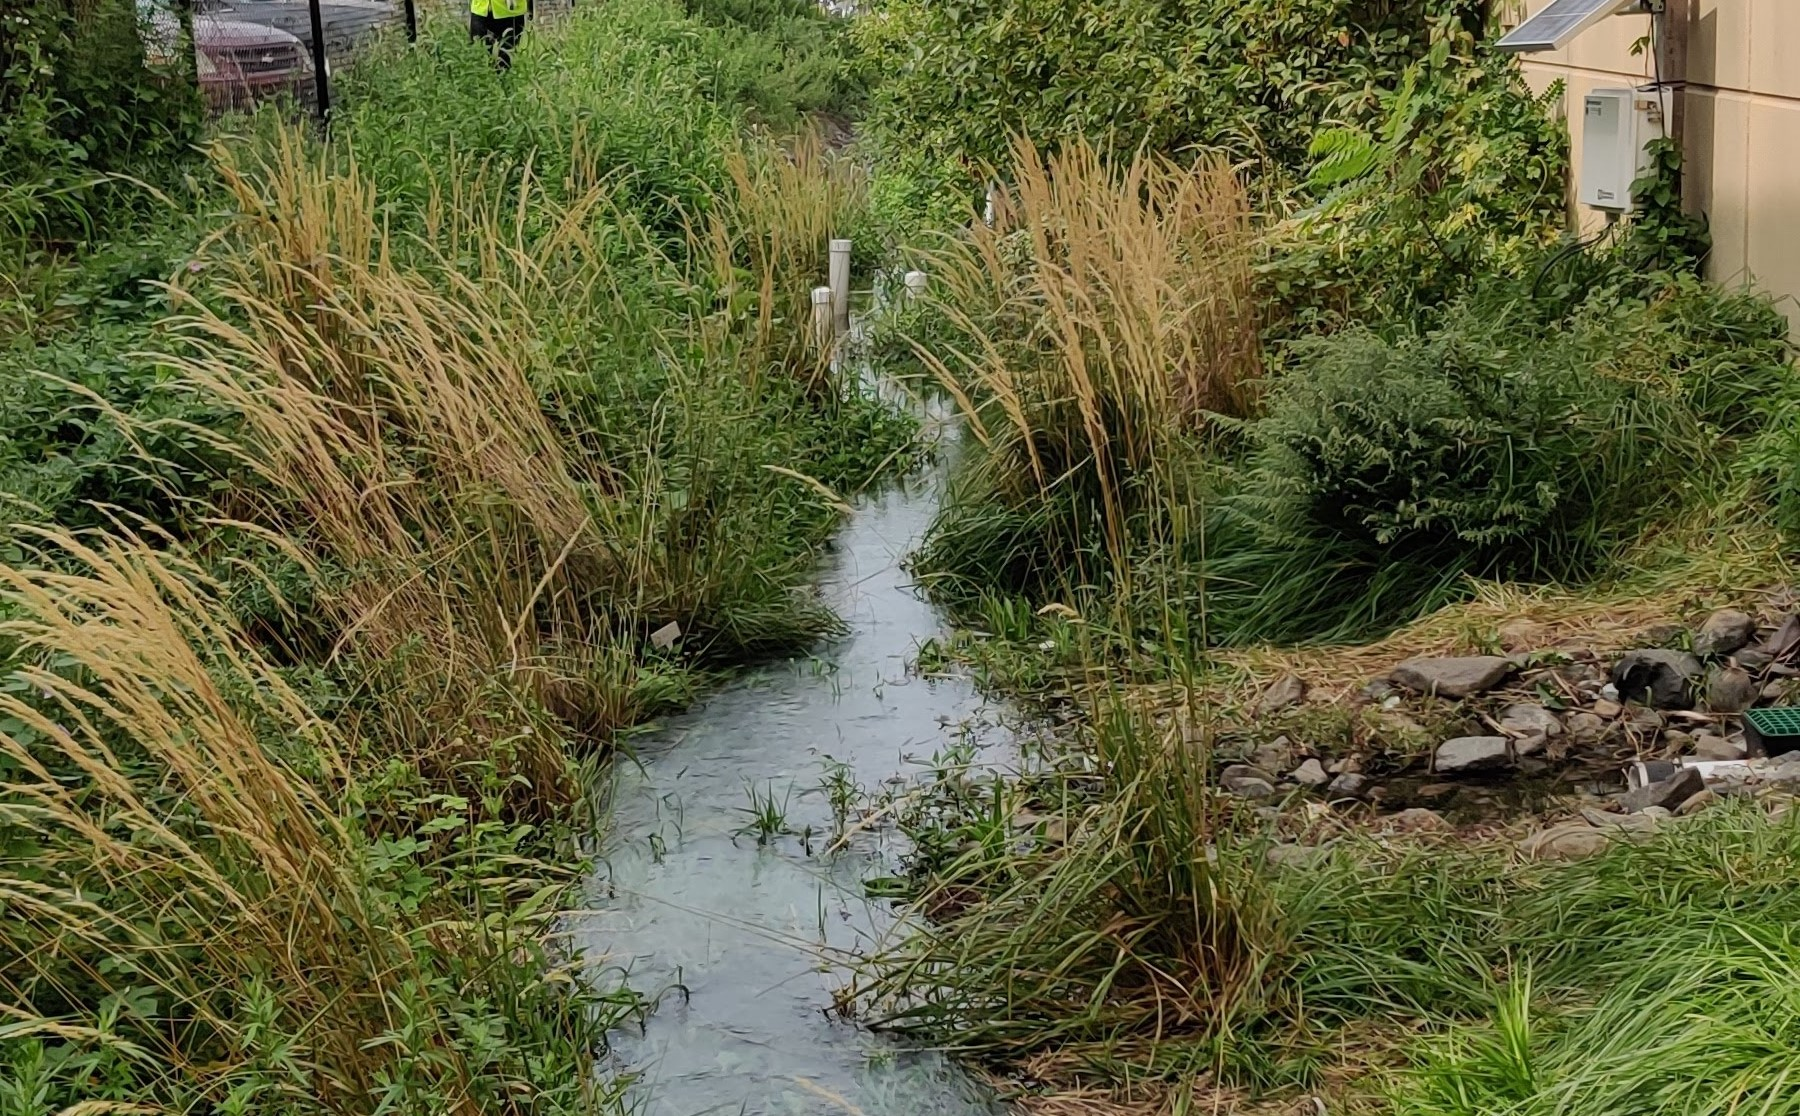
\includegraphics[width=0.4\textwidth]{gfx/chapter-instrumentation/smpa_upstream_profile.jpg}
	\caption[SMP A upstream profile during a simulated runoff test, September 2020.]{SMP A upstream profile during a simulated runoff test, September 2020. Note the shallow side slopes.}
	\label{fig:us-profile}
\end{figure}

\begin{figure}[ht!]
	\centering
	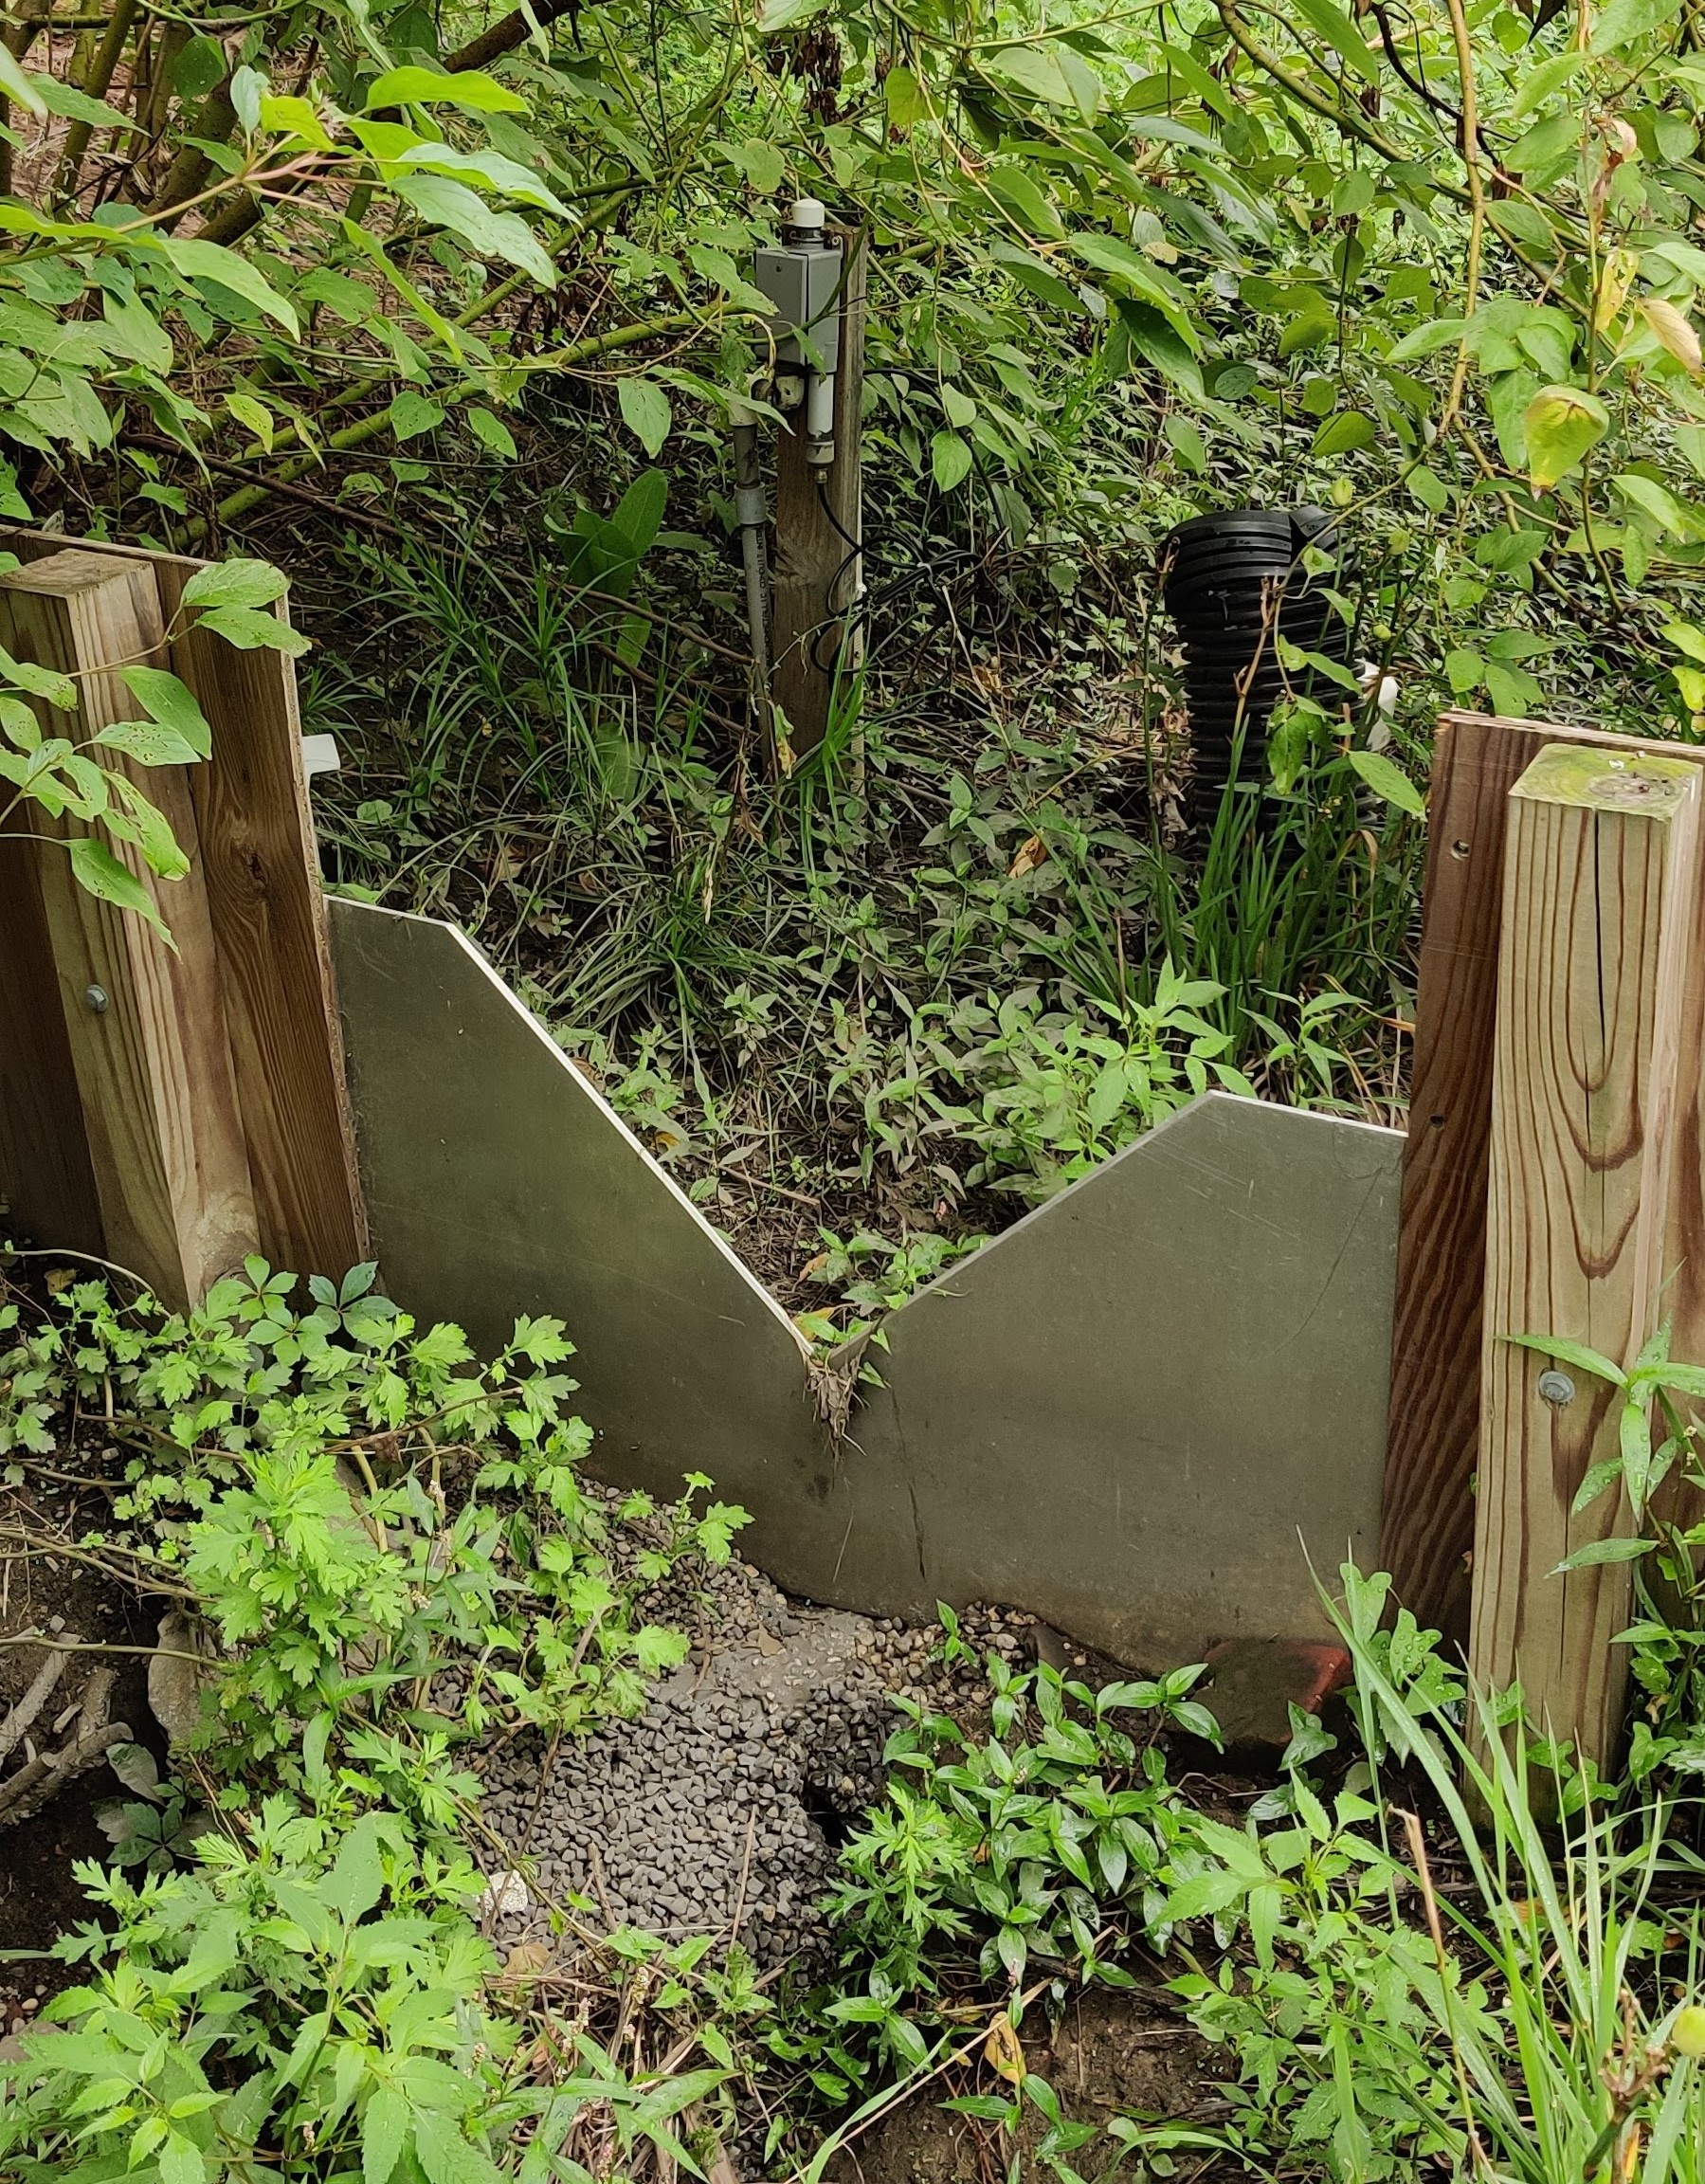
\includegraphics[width=0.4\textwidth]{gfx/chapter-instrumentation/check-dam-weir.jpg}
	\caption{Check dam at the downstream end of the central gabion blanket section of SMP A.}
	\label{fig:check-dam}
\end{figure}

The center section has an impermeable fabric beneath the entire south half of the section to prevent infiltration from damaging neighboring structures' foundations.
The entire section is constructed with gabion basket devices, which are intended to help prevent erosion and cut down on weed growth.
There is a single 45.7cm RCP inlet (N9) in this section and the cross section has more pronounced slopes (Figure \ref{fig:gabion-blanket}).
The gabion blanket section is similarly terminated at the downstream end by a 45\degree\ steel weir plate flush with a check dam to retain as much water as possible.

\begin{figure}[ht!]
	\centering
	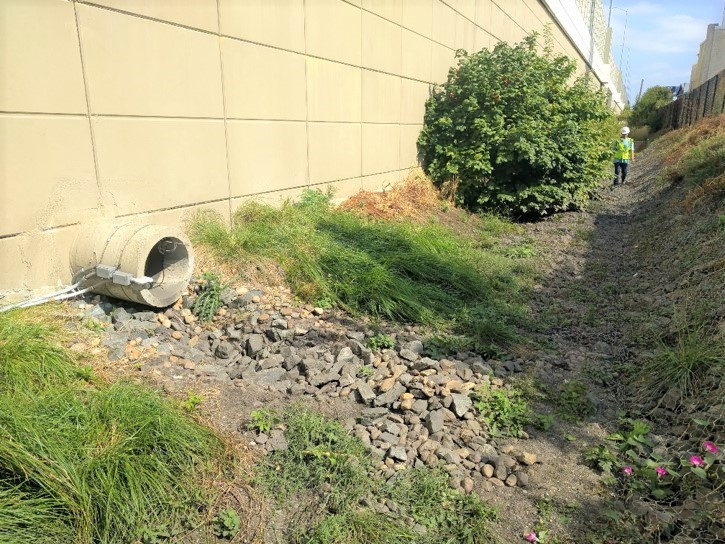
\includegraphics[width=0.6\textwidth]{gfx/chapter-instrumentation/gabion-blanket.jpg}
	\caption{Gabion blanket section showing highly sloped banks.}
	\label{fig:gabion-blanket}
\end{figure}

The downstream portion of the garden contains one more 45.7cm RCP inlet (N10), as well as two concrete overflow structures connected to Philadelphia's CSS identified as B1 and B2.
These structures have pressure transducer (PT) devices attached to the outside of the structure for measuring the ponded water level.
Inside the structures are 22.5\degree\ steel weir plates inside covering the CSS connection (Figure \ref{fig:outlet-structure}), with another pair of PT devices for measuring the outflow from the system, again using the standard weir equation.

\begin{figure}[ht!]
	\centering
	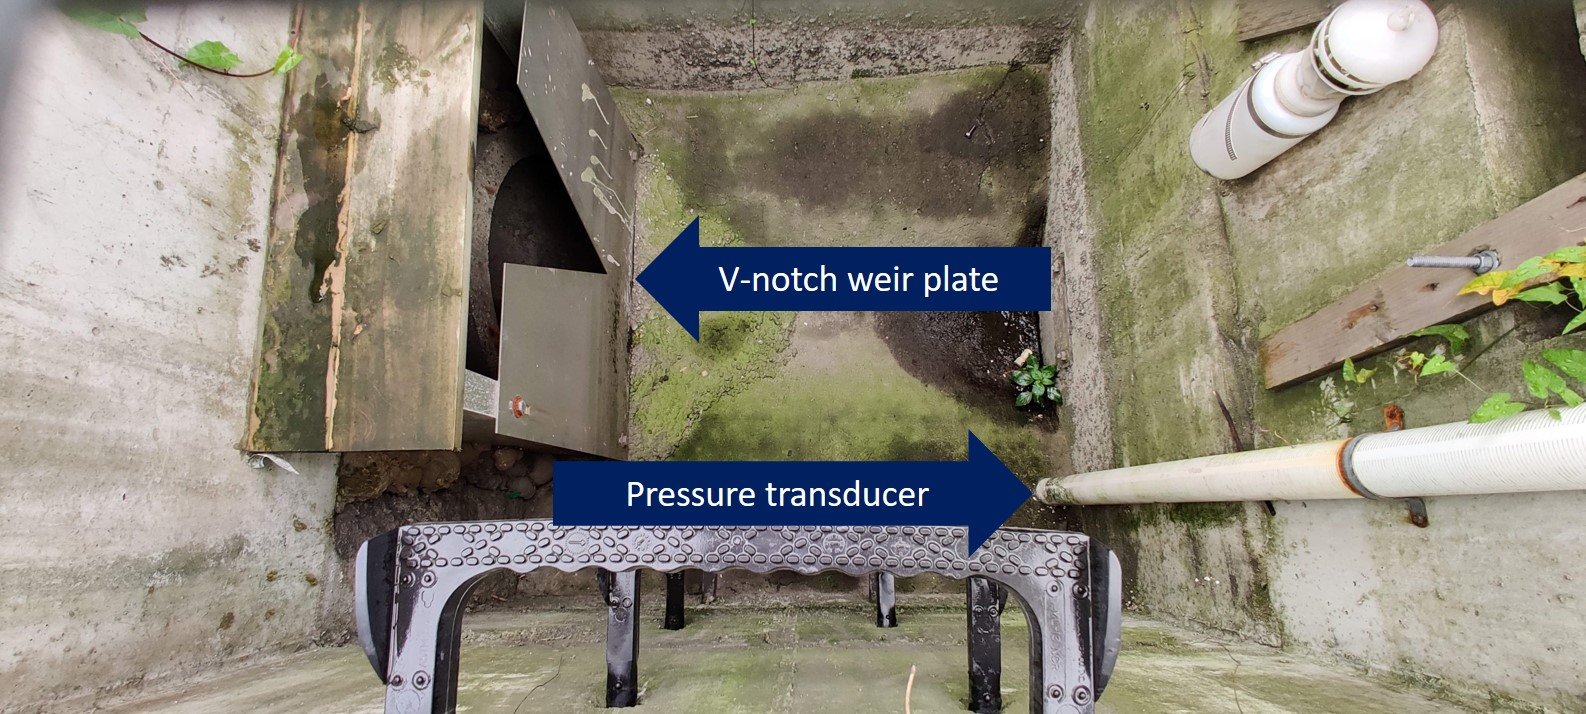
\includegraphics[width=0.8\textwidth]{gfx/chapter-instrumentation/b1-outlet-structure.jpg}
	\caption{B1 outlet structure with weir plate covering CSS connection.}
	\label{fig:outlet-structure}
\end{figure}

Due to SMP A's location at the border between the completed GR2 section of the project and the upcoming GR1 section to the west, there is a temporary construction ramp at the downstream end of the basin that leads from the elevated roadway to grade level adjacent to Frankford Ave.
The ramp is not intended to convey inflow, but the grade of the highway, misalignment of inlet grates (Figure \ref{fig:misaligned-catchments}) on the highway, and lack of barrier at the top of the ramp mean that a substantial amount of runoff enters the basin after flowing down the ramp.
All pressure transducers used at SMP A are a model CS451 digital pressure transducer from Campbell Scientific and are used in their SDI-12 communication mode.

\begin{figure}[ht!]
	\centering
	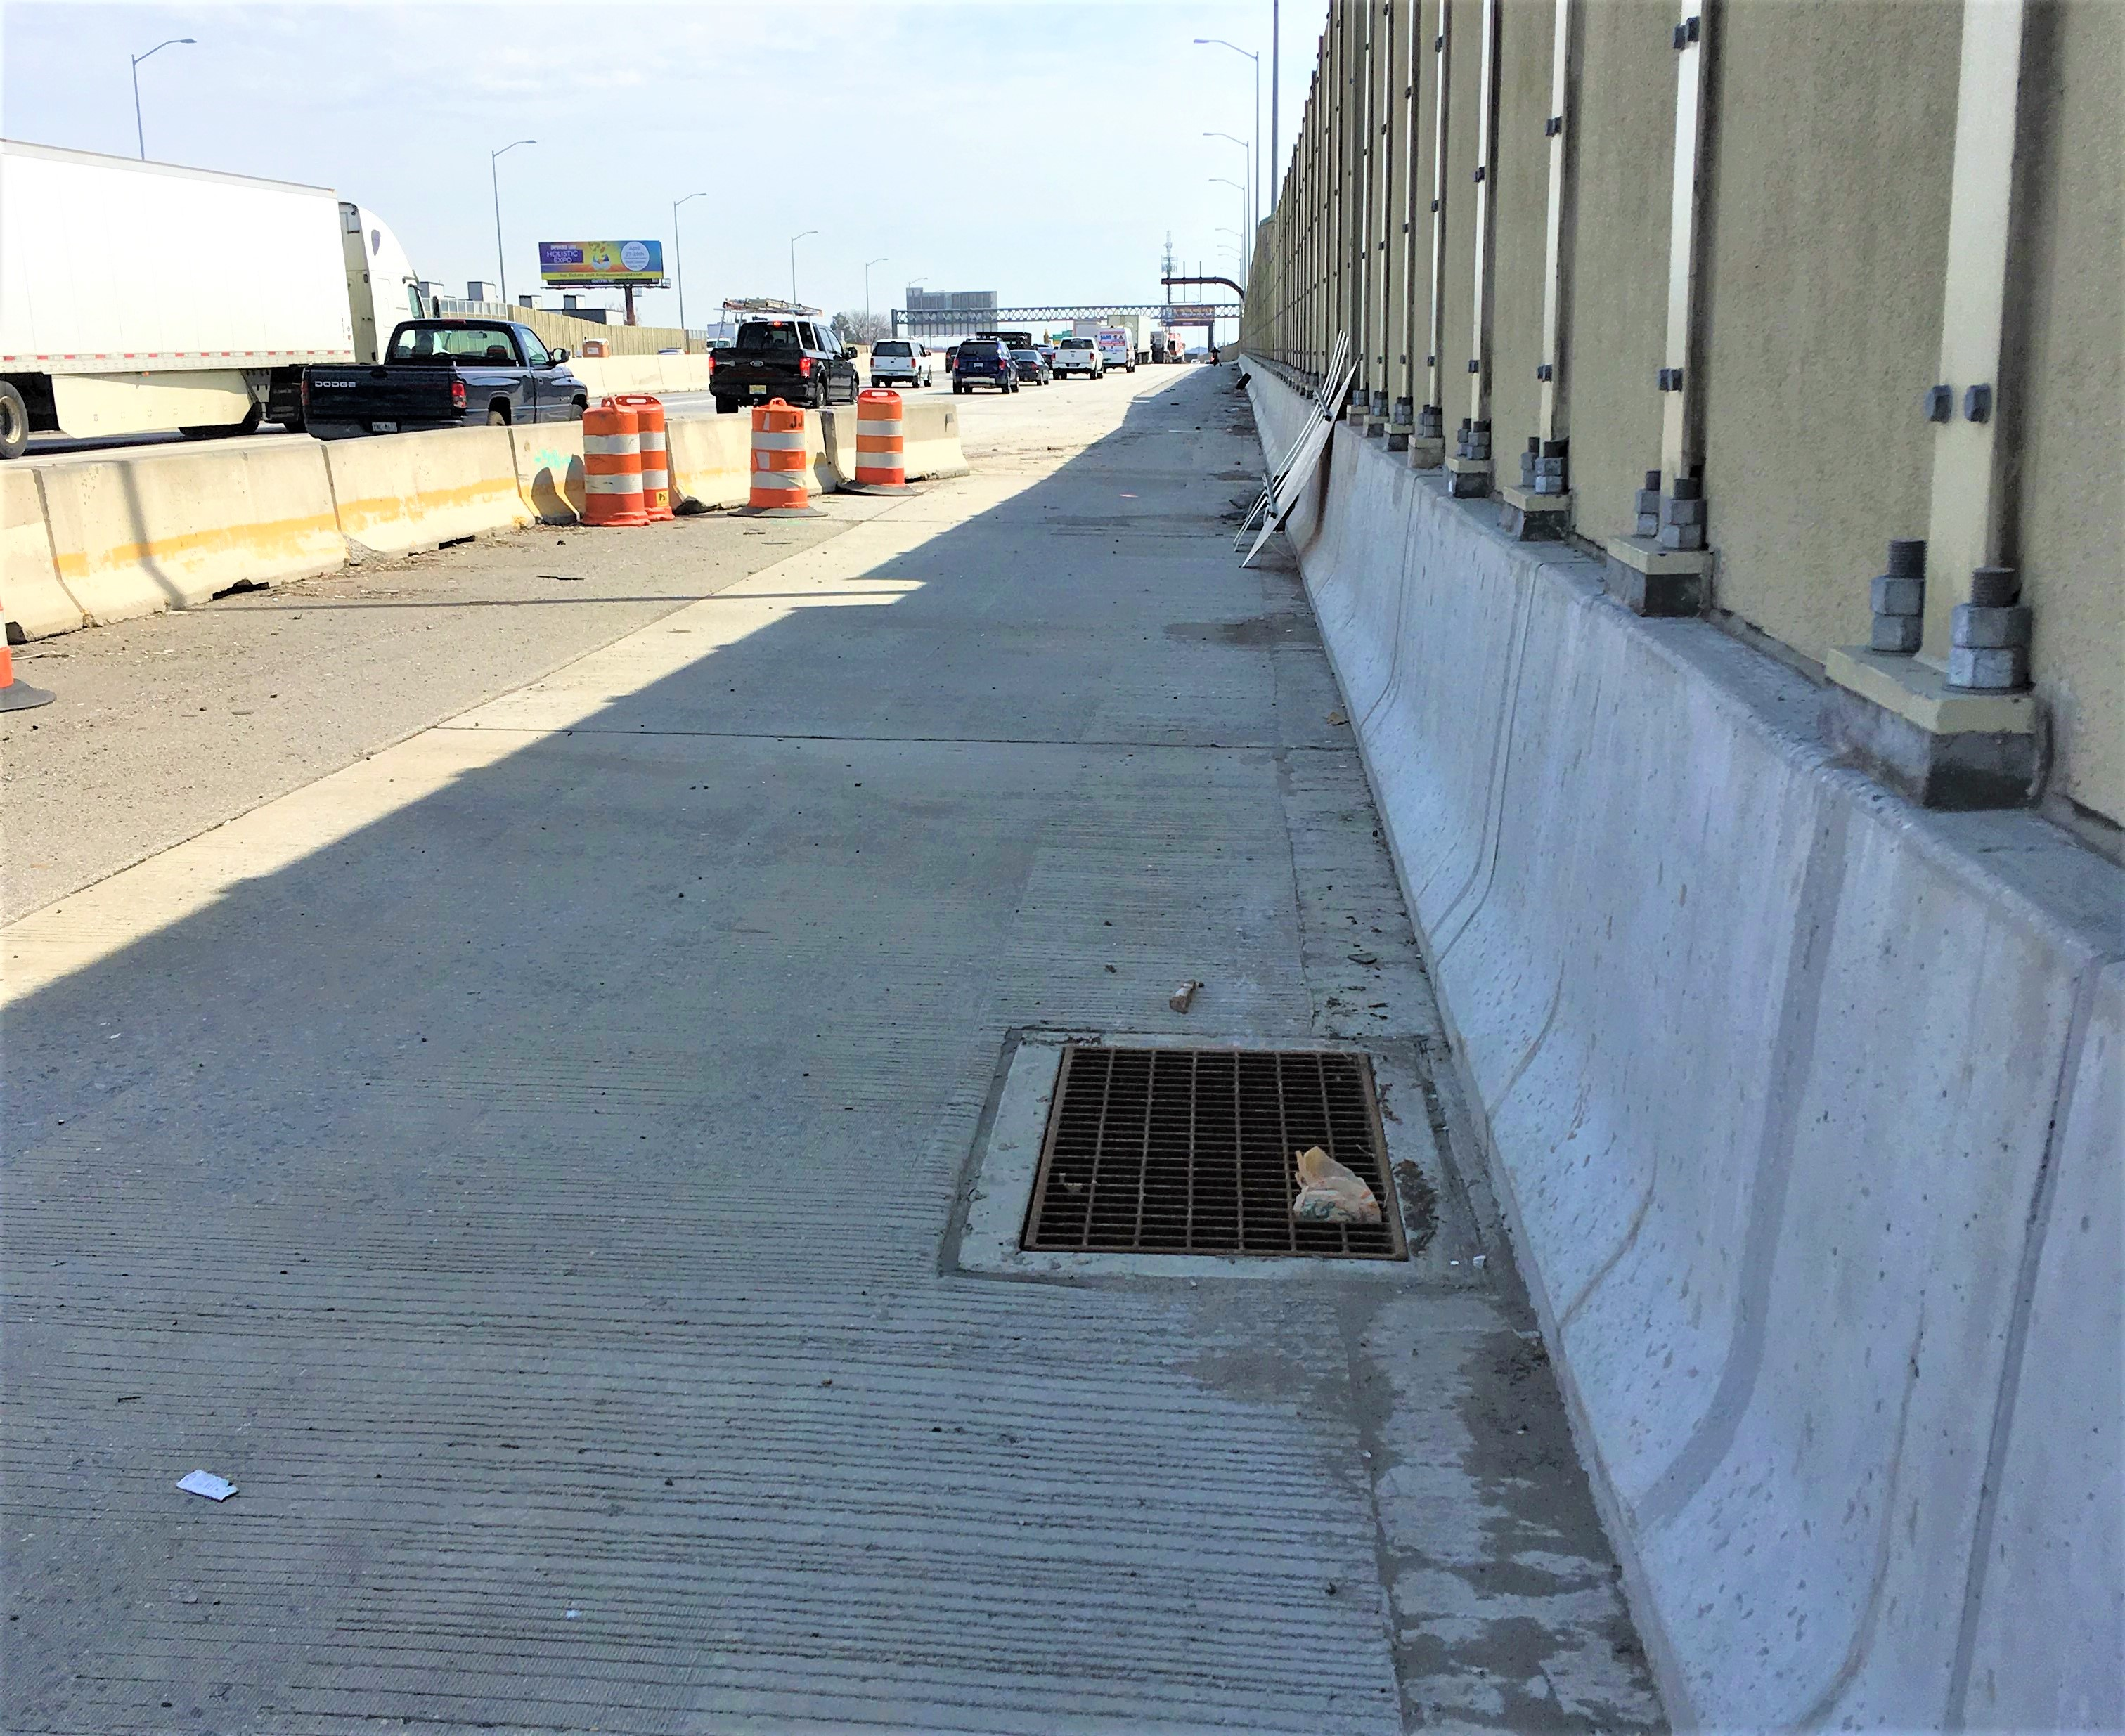
\includegraphics[width=0.6\textwidth]{gfx/chapter-instrumentation/misaligned-catchments.jpg}
	\caption{Misaligned inlet grates allow water to bypass and flow down the temporary ramp.}
	\label{fig:misaligned-catchments}
\end{figure}


\subsection{Measurement: Sensors and Structures}

To aid in repeatable, accurate, and timely measurements, sensors are deployed at a variety of locations throughout SMP A.
Pressure transducers in a variety of locations monitor both ponding level (outside the B1 and B2 outlet structures) and the depth behind weir plates (inside B1 and B2, and behind two check dams separating garden sections).
The flow rate over weir plates can be calculated using the standard weir equation (\cite{USBR2007}).

Inlet flow at N8, N9, and N10 was originally measured by a single BlueSiren Dual Wave Doppler Area-Velocity (AV) sensor at each inlet.
These sensors are fixed to expandable steel bands that secure the apparatus inside the end of the RCP by means of a screw jack.
Located at the downstream end of the AV sensor is a PT that measures flow depth, and outputs a 0-5V analog signal proportionate to the observed depth.
The voltage response must be calibrated with several known depths to establish a valid conversion equation (see section \ref{sec:challenges}).
At the upstream end of the AV sensor, the dual wave doppler measures flow velocity and outputs an 8-bit serial signal, with the number of doppler pulses reflected by the water corresponding to the velocity in millimeters per second.
Both parts of the AV sensor require 12V direct current (DC) power supply, which is managed by the CR6 data logger.

Soil moisture is measured at two locations using sensors at 10cm, 35cm, and 60cm depths, with an additional, redundant sensor at 35cm for quality assurance purposes.
Stevens Water Hydraprobe sensors (Figure \ref{fig:hydraprobe}) are used to measure soil moisture level, conductivity, resistivity, temperature, plus real and imaginary dielectric permittivity.
Hydraprobes use four stainless steel prongs to measure the soil's parameters and "take into account the energy storage and energy loss across the soil area using a 50MHz radio frequency wave" (\cite{StevensWater}).
The sensors are located in the middle of the downstream basin between outlet structures B1 and B2, as well as in the upstream basin approximately 2 meters from the check dam.

\begin{figure}[ht!]
	\centering
	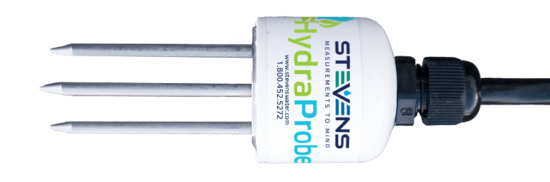
\includegraphics[width=0.6\textwidth]{gfx/chapter-instrumentation/hydraprobe.png}
	\caption[Steven's Water Hydraprobe.]{Stevens Water Hydraprobe (\cite{StevensWater}).}
	\label{fig:hydraprobe}
\end{figure}

Additional climate sensors include air temperature and relative humidity, solar radiation, wind speed and direction, and barometric pressure.
These sensors are located atop a 60-foot telephone pole adjacent to the I-95 bridge over Frankford Avenue that extends roughly 40 feet above the highway surface for measurements uninterrupted by traffic or highway structures.
These sensors are collectively referred to as the "Weather Station," and are a physically separate network from the main garden.

\subsection{Data Collection and Transmission}

The entire sensor network is controlled and monitored by three Campbell Scientific CR6 data logger devices.
These are located on poles attached to the B2 outlet, at the base of the weather station pole, and on a small post in the ground next to inlet N8.
The data loggers are inside protective boxes and have solar panels mounted adjacent to provide power and charge the 12V battery also located in each box.
The CR6 runs a program written in Campbell Scientific's CRBasic programming language, which is a procedural language similar to the BASIC family of languages.
The program defines variables, storage tables, polling and logging frequencies, and monitors the CR6's health and battery status.

Communications at SMP A are achieved via Campbell Scientific's Pakbus protocol, which allows multiple CR6 loggers at one site to be connected via external Wi-Fi modules (model NL240 and NL241) or RF devices (model RF407).
In early 2019, the existing RF devices were swapped out for Wi-Fi devices which improved range, reliability, data link speeds, and security.
Campbell Scientific LoggerNet software is used to remotely manage the data loggers, collect data every three hours, and identify issues that require on-site maintenance.

Remote connections are achieved via a Verizon 4G-LTE cellular modem which provides internet access for remote connections and download of data.
The modem is paired with the CR6 at the Weather Station, as this setup has the fewest instruments attached, and therefore the lowest power requirements.
Remote access is necessary for downloading data at a regular interval and monitoring the network's health.

There are four types of measurement performed by the CR6 data loggers: analog voltage difference, serial, pulse count, and digital.
Each have their advantages and disadvantages.

Analog voltage difference sensors, such as the BlueSiren AV depth reading, convert a 5V or 12V DC supply into a 0-5V response, which is read by the data logging device.
This method requires a calibration equation to translate the response voltage into meaningful units for the measured variable.
The reading is performed by the CR6 device and is almost always separated from the point of measurement (sensor) by a substantial length of wire (minimum 10m, maximum 90m).
Calibration is performed by applying a known reading to the sensor (depth of water in the case of a PT sensor), and recording the response voltage at several different readings.
A linear relationship (slope and intercept) are then calculated from the points collected, and this equation is written directly into the CR6 program.
Due to electrical resistance of copper wire varying with temperature (\cite{Eargle2002}), the resistance of a copper wire increases by 15\% over a 40\degree\ Celsius range when warmed by direct sunlight.
This is amplified by the long length of wire running between the sensors and data logger - nearly the entire 90-meter length of SMP A in some cases.
Change in resistance from the calibration condition is not compensated for by the CR6, so measurements made at temperatures different from the calibration temperature are subject to error.
Historically, wiring has been installed at least partially above ground, exposing it to sunlight which can cause swings in temperature.
Existing in-situ calibration procedures may help reduce this, but further study is warranted.

Serial sensors send pulses of electrical signals at a given voltage and baud rate.
The CR6 data logger reads these serial values by opening a serial buffer on the port a serial sensor is connected to and can respond to a wide variety of serial protocols and refresh rates.
The Blue Siren sensors used at SMP A communicate velocity via UART - TTL at a baud rate of 4800.
Serial communications are less prone to error or disturbance introduced by the transmitting wires but have limits on how far a valid signal will transmit.
Additionally, only one serial sensor can be active on any given data logger port at once, so some inlet AV sensors are connected to switched 12V power outputs on the CR6 to allow multiple sensors to share a single physical port.
This complicates both the physical wiring of the sensors at the site, as well as the code required to handle toggling the power state in coordination with taking measurements.
Additionally, it is unknown what effect this power cycling of the AV sensors has on their performance.

Pulse count communications are used primarily by rain gauges.
Measurement occurs when a specific event happens, such as the tip of a tipping rain gauge.
The sensor briefly connects the measurement port to ground, creating an electrical pulse that is detected by the CR6.
This means pulse count sensors are among the simplest in terms of wiring, as they require only a measurement and ground lead.

Finally, digital sensors, including the CS451 PT, Hydraprobes, pyranometer, and thermometer, use the SDI-12 protocol which allows up to 62 addressed sensors on a single communications port.
The SDI-12 protocol allows the CR6 to poll sensors for up-to-date data on demand, and read the results back nearly instantaneously.
The digital transmission of data eliminates the need to run separate communications cables for each sensor, and consolidates the ports used on a CR6 to just one for most applications.
Sensors are able to relay several measurements to the CR6 in an array of values without concerns surrounding wire length or environmental conditions.

\section{Challenges}
\label{sec:challenges}

Water flowing through pipes or across surfaces is affected by a variety of factors: slope, roughness, temperature, and geometry (\cite{mays2010water}).
The slightest imperfections in the surface or inconsistencies in the roughness can introduce turbulence, a non-uniform flow regime not well suited to measurement by sensors best suited for steady, uniform conditions.
The act of falling from highway level to ground level, where measurement takes place, means that water has a high amount of kinetic energy and is thus more likely to splash around, disturbing calmer water and imparting some of its energy.
Turbulence is best handled by some form of flow straightener, calming device, or impoundment behind a flow-control device such as a weir plate that uses temporarily stored water to remove energy from incoming water.
At lower flow rates, this can also be accomplished through the use of high permeability foam, which has the added benefit of filtering out larger debris particles washed in from the highway surface.

Attempts to characterize the "average" storm year have been successful (\cite{Albright2018}) and provide a means of estimating rainfall over a given period of interest.
This rainfall can be used as the input for a system model, such as was created by Elizabeth Calt, MSCE `18 (\cite{Calt2018}).
The Environmental Protection Agency's (EPA) Stormwater Management Model (SWMM) created by Calt estimates runoff, storage, and overflow volumes and was used to estimate the expected values for the sensors measuring flow through the three RCP inlets during both historical rainfall records, and two design storms (2 year, 24 hour and 10 year, 24 hour).

Historical data from inlet N8, N9, and N10 show that the depth portion of the AV sensors is frequently negative, which is indicative of improper calibration or sensor malfunction.
Despite sensors regularly being calibrated carefully, and returning valid measurements immediately after calibration, measurement drift continues to be an issue.
Little of the data in the period of study is valid, with many negative values occurring during storm events, so the best estimates of inflow rates are from the aforementioned SWMM model developed by Elizabeth Calt.
In addition to negative inflow rates being invalid, the model suggests that flow rates lower than what the Blue Siren AV sensors are capable of detecting may occur frequently, depending on the size and shape of the runoff hydrograph.

Finally, the calibration procedure for existing Blue Siren AV sensors is both tricky to perform and subjective based on human error.
After removing the sensor from the steel band holding it inside the pipe, the sensor is submerged in a five-gallon bucket with water measured by hand to the nearest millimeter.
Simultaneously, the data logger program must be updated to read out the raw voltage received, and these values are recorded in an Excel spreadsheet.
After taking measurements at several depths, typically ranging from 25-150mm, the hand measured depths and corresponding voltages are transformed into a simple linear relationship (slope and intercept), which is then updated and enabled in the data logger's program.
While little to no drift over time is noticeable in historical calibration records, there is some oscillation that occurs do to the imprecision of human measurement during the calibration process.


\section{Solutions}

\subsection{Temporary Ramp}

In June 2019, approximately 60 sandbags were added to an existing asphalt berm on the ramp.
These sandbags were placed to guide water through an 0.8-foot (20.32cm) H-flume with a PT sensor to capture the hydraulics of the ramp (Figure \ref{fig:temporary-ramp}, \cite{OpenChannelFlow2021}).
The flume is sourced from OpenChannelFlow, a company in Boise, ID that focuses on agricultural flow measurement devices.

\begin{figure}[ht!]
	\centering
	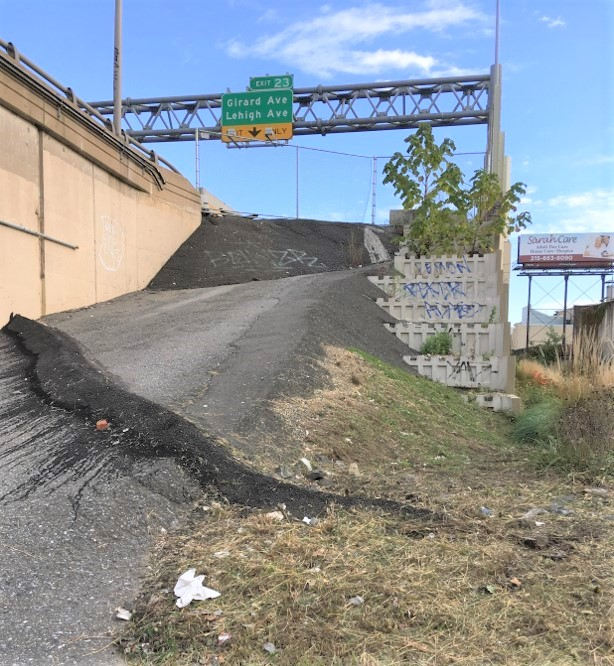
\includegraphics[width=0.6\textwidth]{gfx/chapter-instrumentation/temporary-ramp.jpg}
	\caption{Temporary ramp at the downstream end of SMP A.}
	\label{fig:temporary-ramp}
\end{figure}

The addition of the H-flume near the B1 outlet structure was driven by a desire for better understanding of hydraulic inputs to the basin that were bypassing storm drains on the roadway surface and instead flowing down the temporary ramp.
The H-flume is made of reinforced fiberglass and is sized based on preliminary output from Elizabeth Calt's SWMM model using both design storms and historical rainfall data collected at the site through early 2019.
It has a 1-meter (3-foot) approach section, and two cylindrical measurement wells on either side of the pour point which are 150mm deep (Figure \ref{fig:flume-drawing}).
Using the known offset of these wells, the data recorded by a CS451 PT can be used along with the calibration curve supplied by OpenChannelFlow to establish the flow rates observed:

\begin{equation}
	F = -0.00707921 + 0.04898248\ d^{0.5} + 21.70307374\ d^{1.5} + 365.9132927\ d^{2.5}
\end{equation}

where F is flow in liters per second and d is depth of flow in meters, which gives this flume a range of 0.0085 - 12.94 L/s (\cite{OpenChannelFlow2021}).
Flumes have long been an agriculture industry standard for measuring flows into and out of fields and ponds, and they are well equipped to handle a large range of flow rates.
While the sandbag wall has been tampered with on several occasions, it largely remains intact and able to direct water through the flume (Figure \ref{fig:flume-site-1}).
Only minor leakage was observed during a fall 2020 simulated runoff test (SRT) when a high flow rate was pumped into the site.

\begin{figure}[ht!]
	\centering
	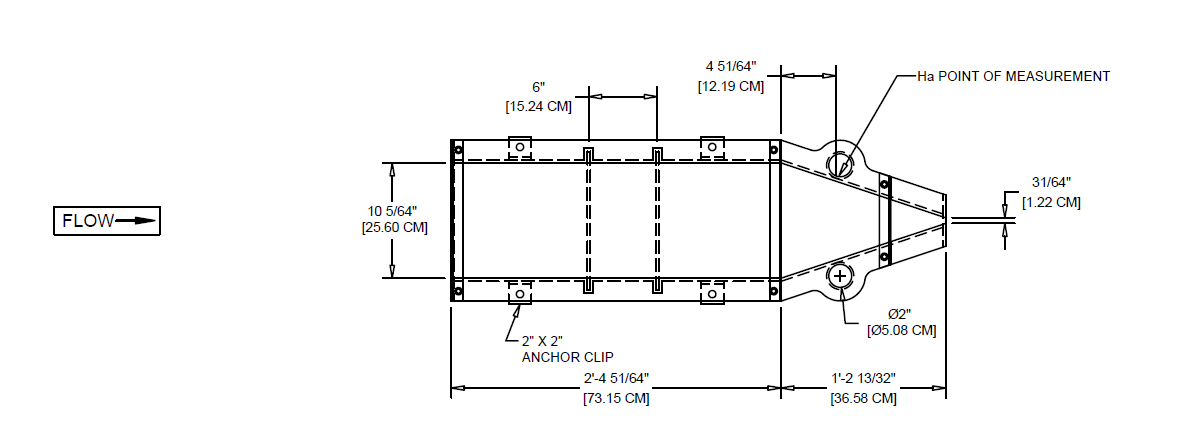
\includegraphics[width=0.8\textwidth]{gfx/chapter-instrumentation/h-flume-plan-view.png}
	\caption[0.8-foot OpenChannelFlow flume plan view.]{0.8-foot OpenChannelFlow flume plan view (\cite{OpenChannelFlow2021}).}
	\label{fig:flume-drawing}
\end{figure}
\begin{figure}[ht!]
	\centering
	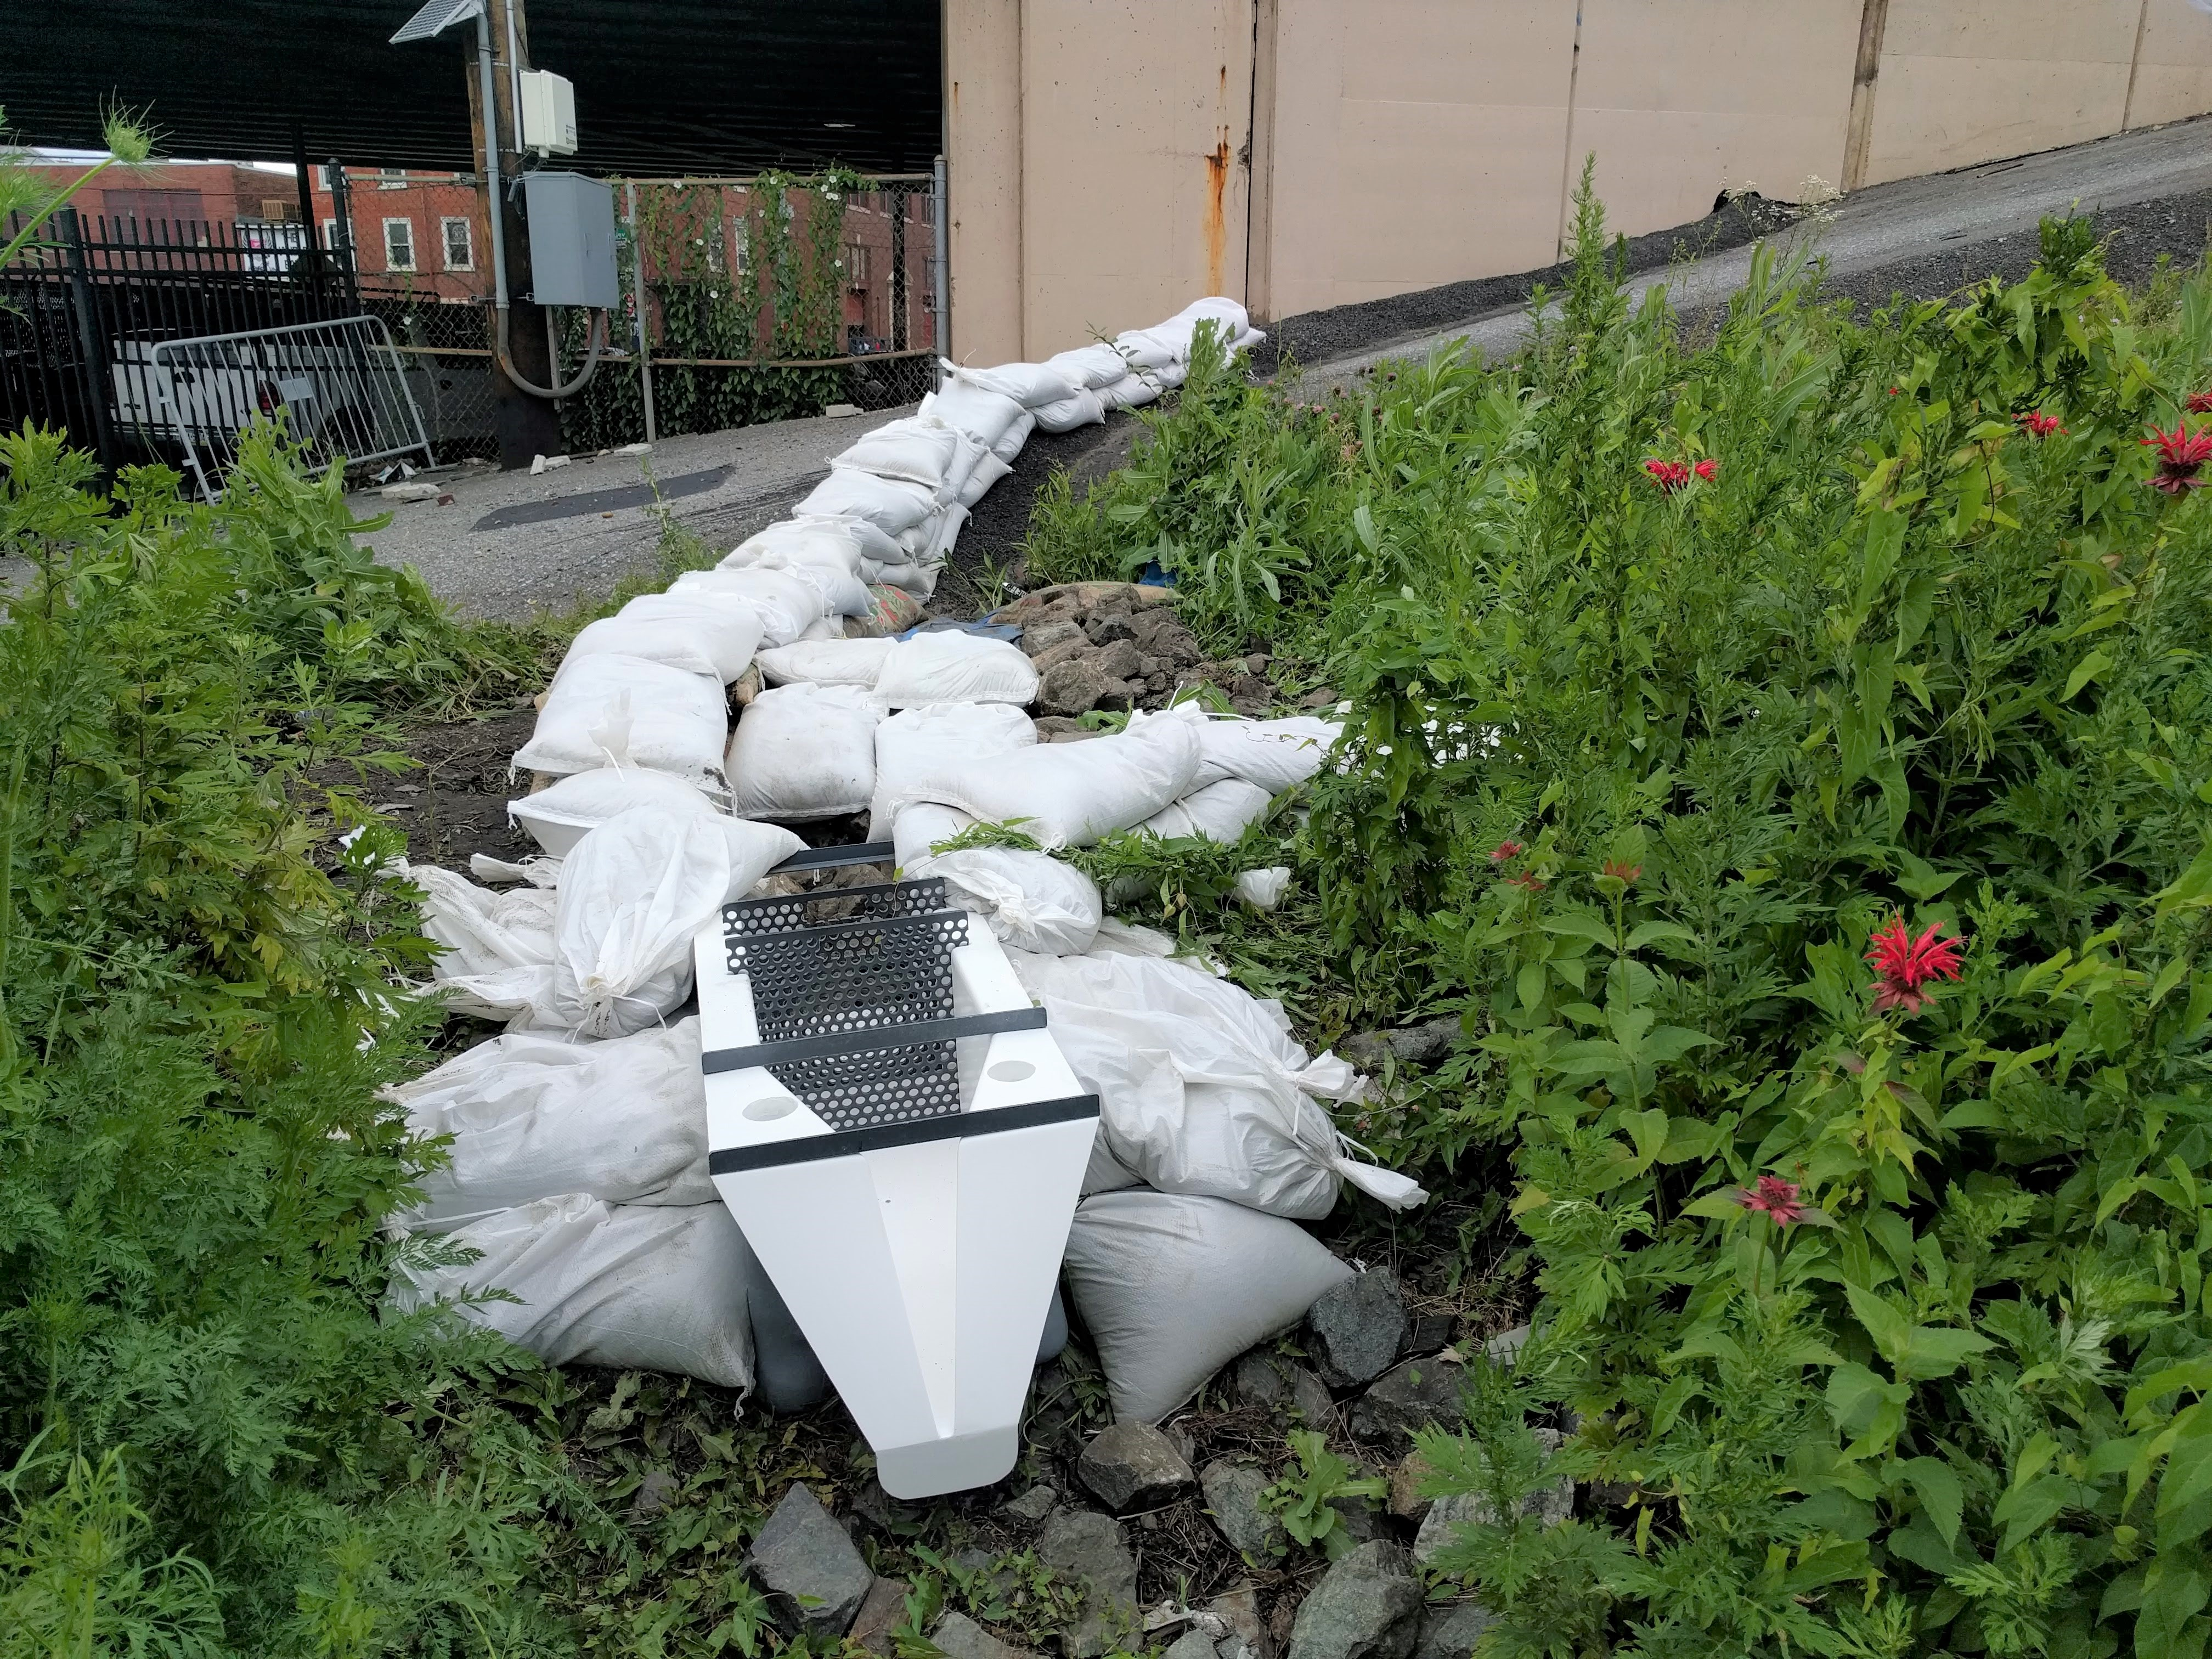
\includegraphics[width=0.6\textwidth]{gfx/chapter-instrumentation/flume-install.jpg}
	\caption{Flume installation at the bottom of construction ramp, 2019.}
	\label{fig:flume-site-1}
\end{figure}

\subsection{Inlet Flow Measurement}

To estimate the AV sensors' range, a suite of tests were performed using a lab simulation of field conditions.
Sensors were attached to an identical steel band and placed inside a 20cm PVC pipe.
The roughness of the pipe is different than that of the RCP installed in SMP A.
However, given the turbulence introduced by the flow falling from highway level to ground level a short distance upstream of the measurement point, roughness does not control the flow profile (\cite{mays2010water}).

The lower bound for Blue Siren AV sensors was determined in Villanova's water resources lab by calibrating a sensor using the same procedures used in the field, and then recording the sensor output and flume flow rate simultaneously.
Analysis showed (Figure \ref{fig:av-lab-results}) that the AV sensors are not valid below 4.5L/s in the 20cm test pipe.
This deviation was found to occur separately in depth and velocity readings around an average of approximately 25mm depth and approximately 30mm/s velocity, which equates to 0.1 L/s in a 45.7cm pipe (N9, N10) or 0.14 L/s in a 76.2cm pipe (N8), although it was not possible to test flow rates this low in the lab.
A second Blue Siren system consisting of a serial ultrasonic depth sensor mounted to the top of the pipe combined with a "microvelocity" sensor that has a lower profile than the current Dual Wave doppler AV sensor was tested in an identical fashion and found to have lower velocity accuracy, but consistently better depth accuracy.
Figure \ref{fig:av-lab-results} compares the two Area-Velocity measurement methods, with the insert at right showing both systems measuring significantly lower than the reference flow rate.
\begin{figure}[ht!]
	\centering
	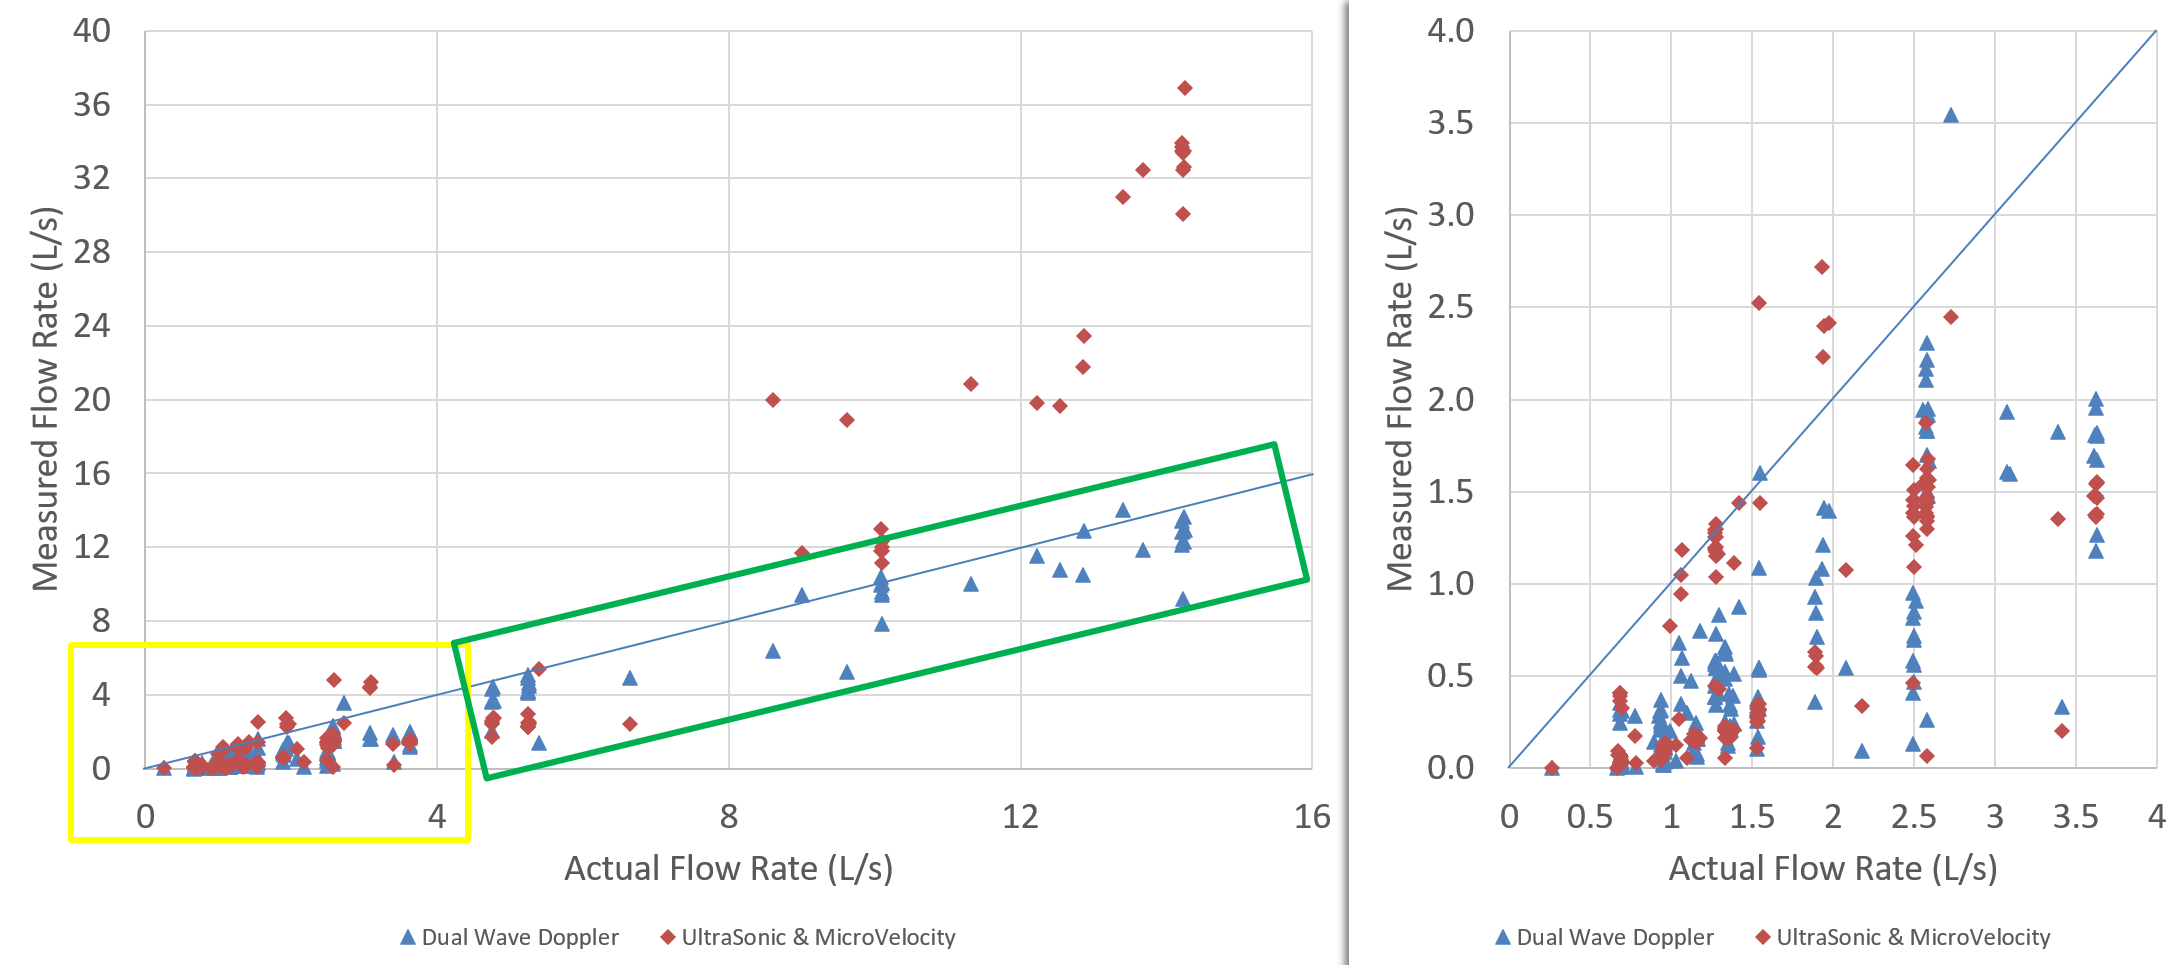
\includegraphics[width=0.8\textwidth]{gfx/chapter-instrumentation/AV-lab-results.png}
	\caption{Area-Velocity measurement comparison results.}
	\label{fig:av-lab-results}
\end{figure}

In order to capture lower flow rates, a restricting structure such as a weir plate or flume is necessary, so that the flow is forced through a narrower opening where it can be measured more precisely.
The solution chosen for implementation is a weir plate sized to fit inside a 10.2cm PVC pipe (Figure \ref{fig:low-flow-setup}), which sits at the outlet of a catch basin small enough to fit under the pour point of the RCP inlets (Figure \ref{fig:low-flow-install}).
This solution minimizes the disturbance to existing infrastructure and involves the least standing water between storms, which is a concern for biological safety during hot summer months.

\begin{figure}[ht!]
	\centering
	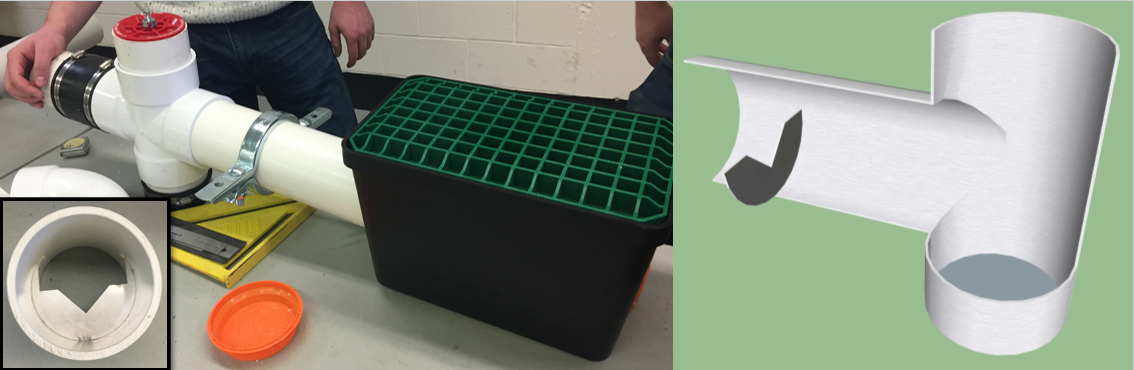
\includegraphics[width=0.8\textwidth]{gfx/chapter-instrumentation/low-flow-setup.png}
	\caption[Low flow measurement setup]{(Left) Low flow measurement setup prototype being constructed in the lab. (Right) Cutaway section of the device outlet.}
	\label{fig:low-flow-setup}
\end{figure}

\begin{figure}[ht!]
	\centering
	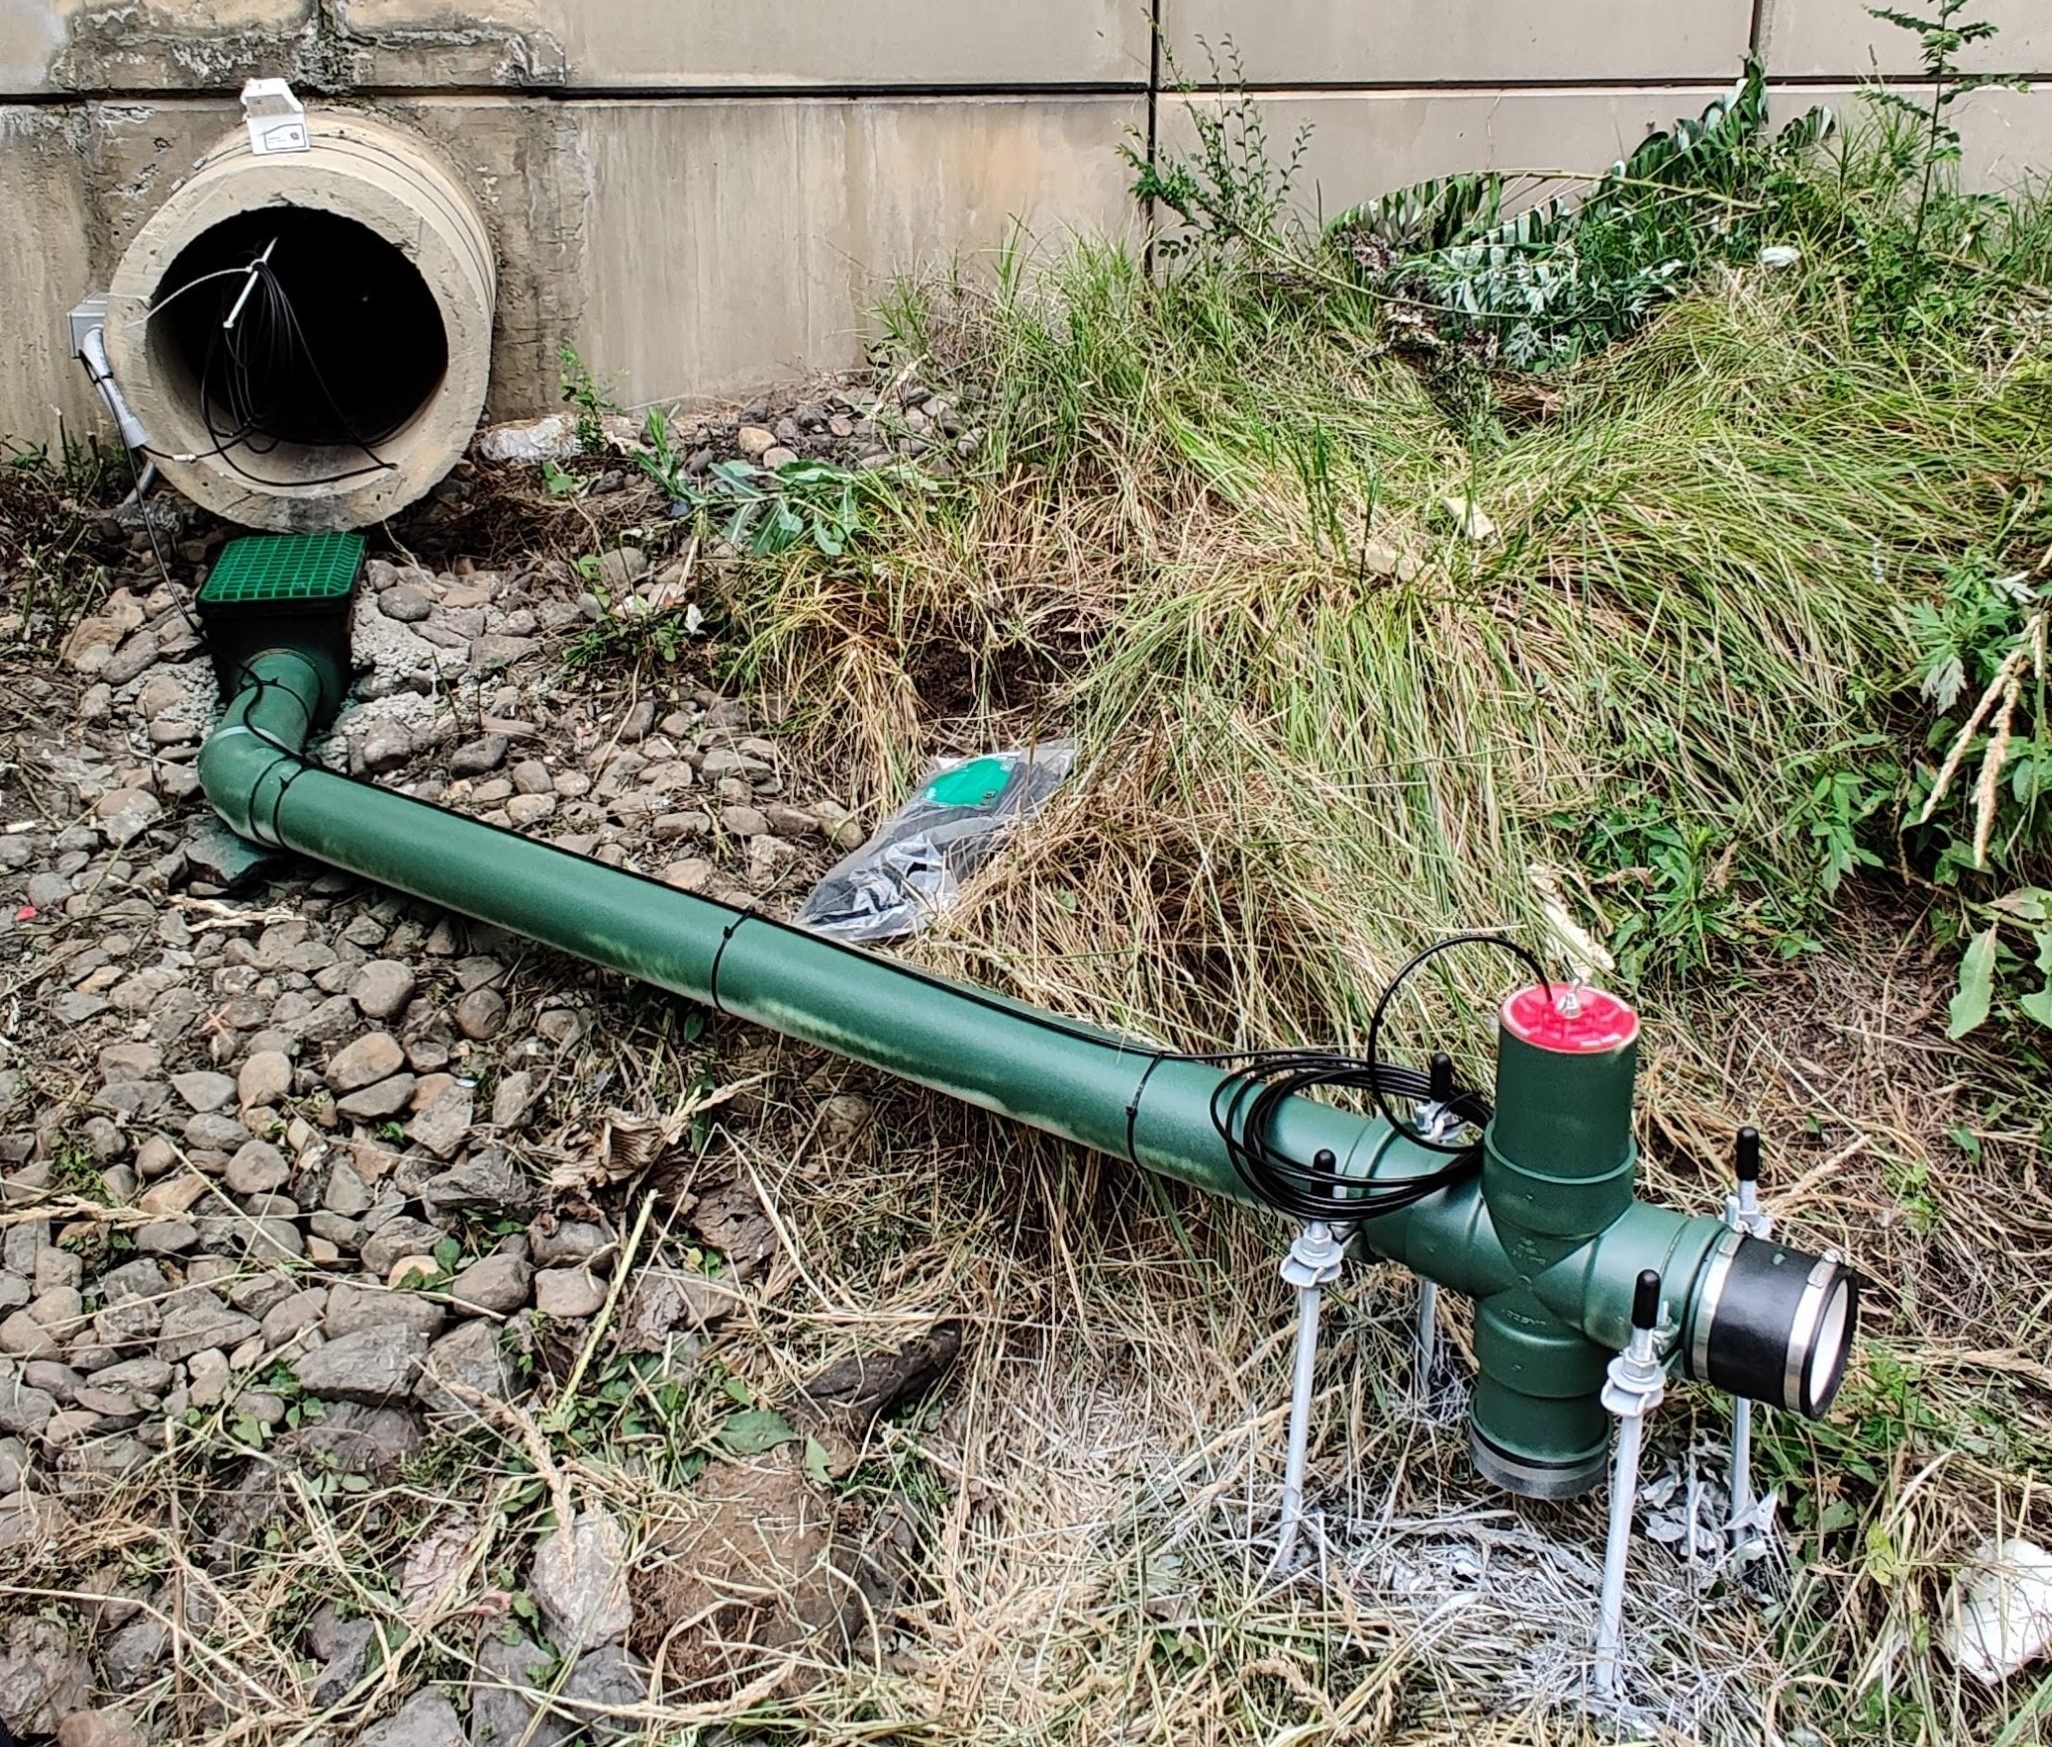
\includegraphics[width=0.6\textwidth]{gfx/chapter-instrumentation/lf-field-install.jpg}
	\caption{Low flow measurement installation.}
	\label{fig:low-flow-install}
\end{figure}

Since installation during summer 2020, the low flow measurement systems at N8, N9, and N10 have captured at least a portion of the flow of each event.
However, several issues remain: the capture efficiency of the inlet (green plastic grate) is lower than anticipated, as a significant percent of flow splashes off and is not captured in the system (Figure \ref{fig:low-flow-splashing}).
Despite this, the inlets show a clear response to rainfall depths as seen in Figure \ref{fig:low-flow-data}.
This data, collected at N9 during a 47mm storm event show a total volume of 3.2$m^{3}$, which equates to just 3.7mm of rainfall over the approximate drainage area of 882$m^{2}$ at N9.
While this could be explained by changes to the drainage area since the LiDAR survey was performed in 2017, bypass due to inlet grate design, or poor capture efficiency at the pour point into the garden, it is evident that the system needs further tuning.

\begin{figure}[ht!]
	\centering
	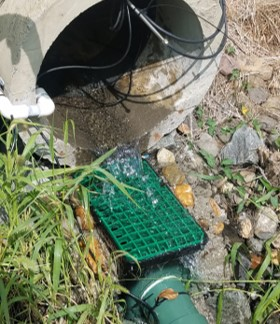
\includegraphics[width=0.5\textwidth]{gfx/chapter-instrumentation/lf-n9-action.jpg}
	\caption{Splashing at N9 low flow installation during September 2020 SRT.}
	\label{fig:low-flow-splashing}
\end{figure}

\begin{figure}[ht!]
	\centering
	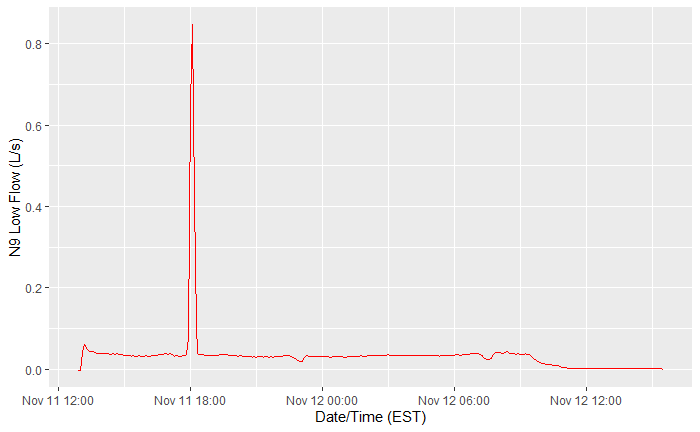
\includegraphics[width=0.8\textwidth]{gfx/chapter-instrumentation/low-flow.png}
	\caption{N9 low flow data for 47mm storm event.}
	\label{fig:low-flow-data}
\end{figure}

\subsection{Future Work}

Investigation into the combination of Blue Siren AV sensor for velocity readings and Massa Ultrasonic depth sensor is ongoing.
Preliminary lab results (Figure \ref{fig:ultrasonic-lab-test-results}) indicate that this system will be sufficiently accurate in combination with the aforementioned low flow system due to their overlap in flow range, shown in orange.

\begin{figure}[h!]
	\centering
	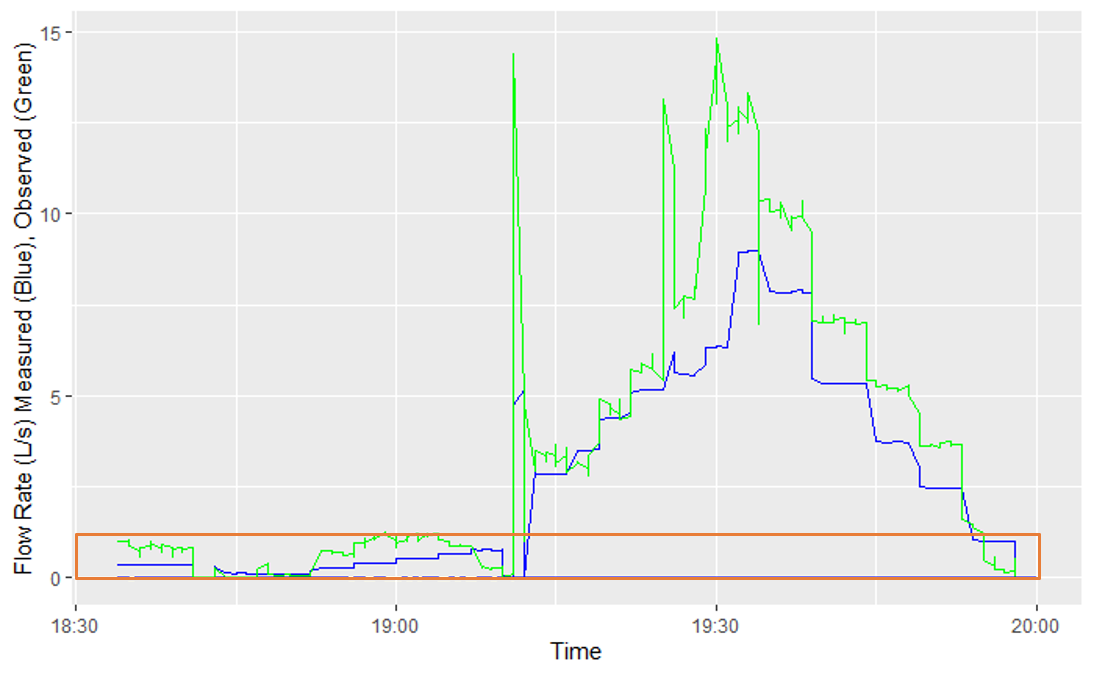
\includegraphics[width=0.8\textwidth]{gfx/chapter-instrumentation/us-flow-test.png}
	\caption{Ultrasonic depth plus Blue Siren velocity preliminary flow comparison.}
	\label{fig:ultrasonic-lab-test-results}
\end{figure}

This system will require further tuning to ensure that the flow rate measurements produced are sufficiently accurate.
The preliminary results show some evidence of hysteresis, when increasing and decreasing flow rates respond differently, but more controlled lab testing is necessary to identify areas for improving this combination of sensors and the CRBasic program that combines the data they produce into a flow rate.
Further testing at more granular flow rates (smaller jumps in flow rate) will help demonstrate whether this system is ready for site implementation.

Finally, due to the variability of analog signal measurement over the long distances in SMP A, conversion to digital measurement will further increase accuracy and reliability.
All lab tests discussed in this chapter have used an analog to digital converter (ADC) between the sensor and data logger as a proof of concept.
The device of choice is a Vegetronix SDI-12 Analog Sensor Translator (Figure \ref{fig:vegetronix}), which supports up to four 0-5V sensors attached and is fully compliant with the SDI-12 protocol.
This inexpensive device will greatly simplify the wiring schematics necessary for using two different sensors (Ultrasonic and AV) for measuring flow at the inlets, as well as shorten the length of wire over which an analog signal must travel.

\begin{figure}[ht!]
	\centering
	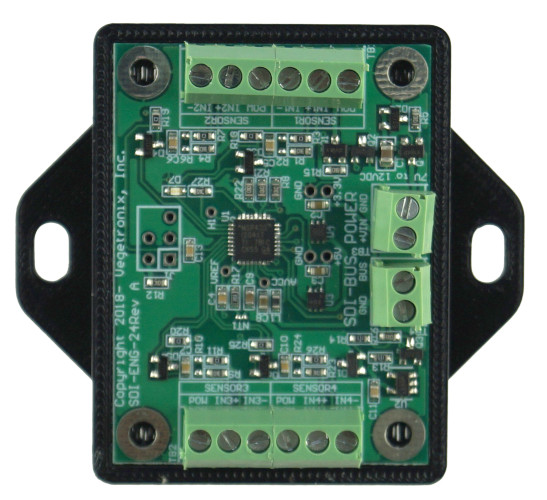
\includegraphics[width=0.2\textwidth]{gfx/chapter-instrumentation/vegetronix-sdi12-converter.jpg}
	\caption{Vegetronix SDI-12 Analog Sensor Translator.}
	\label{fig:vegetronix}
\end{figure}

\section{Conclusions}

Measuring flow in natural, uncontrolled conditions is difficult and requires creativity.
Understanding the intricacies of sensor configurations, communications, randomness of hydraulic characteristics, and opportunities for error can help mitigate invalid data.
Digital communications significantly increase a sensor's ability to report valid data, ensuring that measurements taken in one location are accurately represented and stored by a data logger several hundred feet away.
The increased confidence in data collected will enable future analysis of longer-term trends, so investments and efforts made now in upgrading systems can have lasting benefits for GSI studies across all sites.
Furthermore, significantly less time will be consumed processing the data in quality control procedures leading to more resources available for actual analysis.